\subsection{关于正测度之和的积分}

在本号中，X 表示一个局部紧空间，\((\lambda_{\alpha})_{\alpha\in A}\) 表示 X 上的一个可和正测度族，\(\nu\) 表示测度 \(\sum_{\alpha\in A}\lambda_{\alpha}\) 。

命题 1. --- 设 \(f\) 是定义在 \(X\) 上的一个正数值函数。则

\[
\nu^ {\bullet} (f) = \sum_ {\alpha \in A} \lambda_ {\alpha} ^ {\bullet} (f).\tag{3}
\]

这由注记 1、§1 第 3 号命题 11 及 §1 第 1 号命题 3 立即得出。

推论 1. --- 对 X 的每个紧（相应地，开且相对紧）子集 M，

\[
\nu (\mathrm{M}) = \sum_ {\alpha \in \mathrm{A}} \lambda_ {\alpha} (\mathrm{M}).
\]

推论 2. --- 为使 X 的子集 N 局部 \(\nu\) -可忽略，必须且只须对每个 \(\alpha \in A\) ，N 都是局部 \(\lambda_{\alpha}\) -可忽略的。

推论 3. --- 对每个函数 \(f \in \mathcal{F}_{+}(X)\) ，

\[
\nu^ {*} (f) \geqslant \sum_ {\alpha \in A} \lambda_ {\alpha} ^ {*} (f).\tag{4}
\]

若 \(f\) 不是 \(\nu\) -适度的，则不等式是明显的，因为此时 \(\nu^{*}(f) = +\infty\) （§1 第 2 号命题 7）。若 \(f\) 是 \(\nu\) -适度的，则 \(f\) 是 \(\lambda_{\alpha}\) -适度的（对每个 \(\alpha \in A\) ），因为每个 \(\nu\) -可积开集都是 \(\lambda_{\alpha}\) -可积的；于是关系式 (4) 由 (3) 及 §1 第 2 号命题 7 立即得出。

\pandocbounded{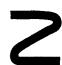
\includegraphics[keepaspectratio]{images/part002_632746ad.jpg}}

即使当 A 可数且每个 \(\lambda_{\alpha}\) 都是点测度时，(4) 的两个成员也可能不相等（ \(\S 1\) 习题 4 \(a\) ））。

命题 2. --- 设 f 是 X 到拓扑空间 G 中的一个映射。为使 f 是 \(\nu\) -可测的，必须且只须 f 是 \(\lambda_{\alpha}\) -可测的（对每个 \(\alpha \in A\) ）。

这由 §1 命题 11 的推论 2 立即得出。

命题 3. --- 为使 X 到 Banach 空间 F 中的映射 f 本质 \(\nu\) -可积，必须且只须 f 本质 \(\lambda_{\alpha}\) -可积（对每个 \(\alpha \in A\) ）且

\[
\sum_ {\alpha \in \mathrm{A}} \int^ {\bullet} | \mathbf {f} | d \lambda_ {\alpha} <   + \infty .\tag{5}
\]

这时族 \((\int \mathbf{f}d\lambda_{\alpha})_{\alpha \in \mathrm{A}}\) 在 \(\mathrm{F}\) 中绝对可和，且

\[
\int \mathbf {f} d \nu = \sum_ {\alpha \in \mathrm{A}} \int \mathbf {f} d \lambda_ {\alpha}.\tag{6}
\]

事实上，为使 \(\mathbf{f}\) 本质 \(\nu\) -可积（相应地，本质 \(\lambda_{\alpha}\) -可积），必须且只须 \(\mathbf{f}\) 对测度 \(\nu\) （相应地，\(\lambda_{\alpha}\) ）可测且 \(\nu^{\bullet}(|\mathbf{f}|) < +\infty\) （相应地，\(\lambda_{\alpha}^{\bullet}(|\mathbf{f}|) < +\infty\) ），这依据 §1 第 3 号命题 9。因而命题的第一部分由命题 2 与命题 1 立即得出。若 \(\mathbf{f}\) 本质 \(\nu\) -可积，则不等式

\[
\sum_ {\alpha \in \mathrm{A}} \left| \int \mathbf {f} d \lambda_ {\alpha} \right| \leqslant \sum_ {\alpha \in \mathrm{A}} \int | \mathbf {f} | d \lambda_ {\alpha} = \nu (| \mathbf {f} |)
\]

表明族 \(\left(\int\mathbf{f}d\lambda_{\alpha}\right)\) 在 F 中绝对可和，且和的范数小于或等于 f 在 \(\overline{\mathcal{L}}_{\mathrm{F}}^{1}(\nu)\) 中的范数。于是满足 (6) 的 \(\mathbf{f}\in\mathcal{L}_{\mathrm{F}}^{1}(\nu)\) 所成之集是 \(\mathcal{L}_{\mathrm{F}}^{1}(\nu)\) 的一个闭线性子空间 H；而这个子空间在 \(\mathcal{L}_{\mathrm{F}}^{1}(\nu)\) 中也是稠密的，因为它包含形如 \(f\cdot a\) 的函数，其中 \(a\in F\) 而 f 表示一个有限可积的正函数（命题 1）。因此 \(\mathcal{H}=\mathcal{L}_{\mathrm{F}}^{1}(\nu)\) ，命题得证。

命题 3 也可由将在 §3（第 3 号定理 1）中证明的关于积分的一般定理导出。

推论 1. --- 设 f 是 \(\nu\) -可积的；则 f 是 \(\lambda_{\alpha}\) -可积的（对每个 \(\alpha \in A\) ），且公式 (6) 成立。反之，若集 A 有限且 f 是 \(\lambda_{\alpha}\) -可积的（对每个 \(\alpha \in A\) ），则函数 f 是 \(\nu\) -可积的。

若 \(\mathbf{f}\) 是 \(\nu\) -可积的，则 \(\mathbf{f}\) 本质 \(\nu\) -可积且 \(\nu\) -适度（§1 第 3 号命题 9 的推论）；因而 \(\mathbf{f}\) 是本质 \(\lambda_{\alpha}\) -可积、\(\lambda_{\alpha}\) -适度从而 \(\lambda_{\alpha}\) -可积的（对每个 \(\alpha \in A\) ）。反之，若 \(A\) 有限且 \(\mathbf{f}\) 是 \(\lambda_{\alpha}\) -可积的（对一切 \(\alpha \in A\) ），则由命题 3，\(\mathbf{f}\) 本质 \(\nu\) -可积，且只需验证 \(\nu^{*}(|\mathbf{f}|) < +\infty\) ；这由关系式 \(\nu^{*} = \sum_{\alpha \in A} \lambda_{\alpha}^{*}\) （第四章，§1 第 3 号命题 15）立即得出。

推论 2. --- 设 \(\theta\) 是 X 上的一个复测度；令 \(\theta_1 = (\mathcal{R}\theta)^+\) ，\(\theta_2 = (\mathcal{R}\theta)^-\) ，\(\theta_3 = (\mathcal{I}\theta)^+\) ，\(\theta_4 = (\mathcal{I}\theta)^-\) 。为使 X 到拓扑空间 G（相应地，到 Banach 空间 F）中的映射 \(f\) 对测度 \(\theta\) 可测（相应地，本质可积、可积），必须且只须它对诸测度 \(\theta_i\) （ \(i = 1,2,3,4\) ）中的每一个都可测（相应地，本质可积、可积）。

若 f 对 \(\theta\) 可测（相应地，本质可积、可积），则按定义 f 对测度 \(|\theta|\) 可测（相应地，本质可积、可积），从而对诸测度 \(\theta_{i}\) （它们都 \(\leqslant |\theta|\) ）也可测（相应地，本质可积、可积）。反之，若 f 对诸测度 \(\theta_{i}\) 可测（相应地，本质可积、可积），则命题 2（相应地，命题 3、命题 3 的推论 1）蕴含 f 对测度 \(\theta_{1} + \theta_{2} + \theta_{3} + \theta_{4}\) （它 \(\geqslant |\theta|\) ）可测（相应地，本质可积、可积）。

